\chapter{Methodology} 
\label{chap:methodology}
This chapter describes the experimental setup used to evaluate the \acrfull{s6} model for temporal event spotting in football video. The section details computing infrastructure, data preprocessing and feature extraction pipeline, model architectures, training protocols, and evaluation metrics aligned with the research questions (\autoref{sec:research_questions}).


\section{Tools and Resources}
\label{sec:tools_and_resources}

\subsection{IDUN}
\label{ssec:idun}
Video processing pipelines demand substantial computational resources. To address this, I utilized the IDUN cluster\footnote{\url{https://www.hpc.ntnu.no/idun/}}. IDUN is a faculty-operated system at NTNU equipped with 234 NVIDIA GPU accelerators (as of April 24, 2024). Although IDUN is not NTNU’s central supercomputer, its nodes, featuring Tesla H100 and A100 GPUs, with up to 80 GB of RAM—provided the necessary throughput for feature extraction and model training. To mitigate occasional queuing delays and VRAM limitations, full-match videos were partitioned into fixed-duration clips and distributed workloads across multiple GPUs via data-parallel training.

Due to the high memory requirements of the \acrlong{tdeed} and software requirements of the \acrlong{s6} framework, all experiments were run on IDUN nodes equipped with modern NVIDIA GPUs. Attempts to train on GPUs with 16 GB of memory triggers out-of-memory errors on occasion with \acrshort{tdeed}. Moreover, MAMBA \acrshort{s6} requires certain CUDA versions and matching libraries, which older driver stacks do not support out of the box. To guarantee stable training and reproducible results, model development and evaluation to was restricted to nodes meeting these hardware and software requirements. 
% later was run on all types of GPU I have no reason how. 

% \subsection{draw.io}
% \label{ssec:draw.io}
% For the creation and maintenance of all schematic overviews—such as model architectures, data‐flow pipelines, and experimental workflows—we employed draw.io (diagrams.net). draw.io is an open-source, web-based diagramming tool that allows rapid assembly of vector‐based figures using a rich library of shapes, connectors and templates. Its native XML file format preserves editability and version history, facilitating collaborative revisions via version control, while export to PDF and SVG ensures high‐resolution inclusion in the thesis document. By standardizing figure style and layout across chapters, draw.io helped maintain visual consistency and improved the clarity of complex methodological and architectural descriptions.

\subsection{\acrfull{wandb}}
\label{ssec:wandb}
To streamline the management and reproducibility of the training experiments, I used the \acrlong{wandb} platform. Using \acrshort{wandb}’s Python client, hyperparameters are logged automatically. As is training and validation metrics, model checkpoints, and GPU utilization statistics. The centralized dashboard enabled real-time monitoring and direct comparison of concurrent runs. Crucially, \acrshort{wandb}’s automated hyperparameter sweep feature was used to conduct systematic searches over predefined parameter distributions. These sweeps coordinated parallel trials, performance metrics, and ranked configurations based on validation outcomes. By integrating \acrshort{wandb} into the workflow, it significantly enhanced the transparency, comparability, and reproducibility of the experimental pipeline.

\subsection{Bayesian Hyperparameter Search}

Bayesian optimization is a probabilistic approach to hyperparameter tuning that efficiently explores the search space by balancing **exploration** (trying new regions) and **exploitation** (focusing on promising regions). It builds a **surrogate model**, typically a **Gaussian Process**, to approximate the objective function and predict both the mean and variance of the function.

The optimization process follows these steps:
\begin{itemize}
    \item \textbf{Surrogate Model}: A probabilistic model estimates the objective function based on previous evaluations.
    \item \textbf{Acquisition Function}: Determines the next hyperparameter set to evaluate by optimizing a function such as **Expected Improvement (EI)** or **Upper Confidence Bound (UCB)**.
    \item \textbf{Evaluation and Update}: The chosen hyperparameters are tested, and the surrogate model is updated with new information.
    \item \textbf{Iteration}: The process repeats until convergence or a stopping criterion is met.
\end{itemize}

Bayesian optimization is particularly useful for tuning hyperparameters in deep learning models, where evaluating each configuration is computationally expensive. By leveraging probabilistic modeling, it efficiently identifies optimal hyperparameter values while minimizing unnecessary evaluations.

\subsection{Comparing Correlation and Importance}

While correlation identifies linear dependencies, importance accounts for complex interactions among multiple hyperparameters. This distinction helps researchers make informed decisions when designing hyperparameter search strategies. Bayesian optimization further enhances this process by intelligently selecting hyperparameters based on probabilistic predictions, leading to improved model performance and faster convergence.

\subsection{Anaconda and pip}
\label{ssec:conda_pip}
Python environments were managed using conda, but all packages—including CUDA-enabled PyTorch builds—were installed via pip to follow recent PyTorch recommendations favoring pip over conda for GPU support.

\section{Data Preprocessing \& Feature Extraction}
\label{sec:preprocessing}

Experiments are conducted on the SoccerNet-V2 dataset\cite{deliege_soccernet-v2_dataset_2021}. Videos are split into non-overlapping clips $V_k=\{x_t\}_{t=1}^{T_c}$ of fixed duration $T_c=60\!\times\!25$ frames (60\,s at 25\,fps). A 70-30 split and an 80-20 respectively for training and validation was used. The 80-20 split matches the official publication. 70-30 matches a PyTorch recommendation in the docs
\footnote{
\url{https://docs.pytorch.org/docs/stable/data.html}. 
Retrieved 13th of May}
.

% 70\% of matches for training and 30\% for validation were initially used. Later on a 80\%/20\% split was favored as it matched the video splits in the original dataset


\unsure{simplify the code and make it shorter. only post relevant sections? (remove classes, try except, imports etc}
\info{This code listing is very long. Maybe appendix?}
\lstinputlisting[
    caption={Script to change the label-file to the THUMOS-14 format.},
    label=lst:jsonfile,
    language=Python
]{listings/sn_to_json.py}
% the next section is how the raw videos are transformed. 
\todo{also trained with 0.8 split and got better result}

\unsure{the code uses random.random to create a train/val split. to reproduce, should I upload the used data for reproducibility?}

Each full‐match video is split into non‐overlapping clips of fixed duration (60 s). Clips are sampled at 25 fps and stored as input sequences $V_k=\{x_t\}_{t=1}^{T_c}$ where $T_c=60\times25$. \todo{edge cases(end of game)}. The duration key is unnecessary in the case of temporal action localization, as shown in the \autoref{lst:uselessduration} which sets a default value if the duration is not explicitly set. 

\lstinputlisting[
    caption={Part of \acrshort{vms} code used to determine the duration to be pointless. },
    label=lst:uselessduration,
    language=Python
]{listings/useless_duration.py}

Each clip $V_k$ is fed through the pre‐trained VideoMAE-V2 encoder (\autoref{ssec:videomae_v2}) to extract a feature embedding
\[
z_k = \mathrm{VideoMAE\text{-}V2}(V_k)\;\in\;\mathbb{R}^D.
\]
These $D$‐dimensional vectors serve as inputs to the downstream  temporal MAMBA-model. The vectors are saved on IDUN as \textit{*.pt} files. This avoids redundant computations, reduces storage requirements and lowers training times significantly. 

Edge‐case handling at the end of match videos was approached by fixed‐length segmentation, despite the model’s capacity to process variable‐length inputs. This simplified protocol was adopted in the absence of established guidelines for optimally splitting football footage. \info{in the literature study i did i found nothing about this} Future research could explore overlapping windows, adaptive clip boundaries, or dynamic segmentation schemes to mitigate boundary artifacts and potentially improve temporal event localization. \unsure{write about future work here and in the end or only in the end}

Despite its demonstrated effectiveness in learning rich spatiotemporal representations, \acrlong{vmae} incurs substantial computational overhead that must be managed in large-scale experiments. The dual-stage masking strategy, in which up to 90 \% of video tokens are hidden during training, yields robust feature embeddings. But, it also increases the number of model parameters and the complexity of each forward pass. In practice, processing a single 60 s clip at 25 fps requires on the order of tens of gigaflops\cite{wang_videomae_2023}. To mitigate these resource requirements, all \acrlong{vmae} embeddings are extracted and stored offline. The heavy compute footprint of \acrlong{vmae} motivates the exploration of more lightweight architectures or more aggressive token reduction techniques in future work. \unsure{again future work}

\acrlong{vmae} has been pre-trained on the large-scale Kinetics dataset\todo{write about kinetics dataset in background}, which comprises thousands of general sports clips over diverse action categories\todo{remove after written background}. Consequently, its learned representations which capture broad spatiotemporal patterns common to various athletic activities, but are not tailored specifically to football. While this generic pretraining supports robust feature extraction across multiple sports domains, specialized fine-tuning on football video may further improve temporal event localization performance. Future work should explore domain-specific adaptation using dedicated football datasets to bridge the semantic gap between Kinetics pretraining and match-level footage. 

InternVideo serves as the foundation for our comparative experiment, in which we evaluate 1,408-dimensional feature vectors extracted by a Kinetics-pretrained model against 3,302-dimensional embeddings generated by an expanded masked autoencoder. Both architectures originate from the same research group responsible for developing VideoMAE-V2. InternVideo is a bigger, still open source framework.

\todo{The weights from internvideo 2 is available for download from huggingface, link is findable. also vectors used in experiments}

\section{Datasets}
\label{sec:method_datasets}

\subsection{THUMOS-14}

\subsection{SoccerNet-V2}

The SoccerNet-V2 dataset \cite{deliege_soccernet-v2_dataset_2021} contains video recordings of 7 professional football matches with fine-grained annotations for 12 action classes. It provides:
\begin{itemize}
    \item 7 full matches (90 min each) at 25 fps.
    \item Time-stamped action labels for spotting tasks.
    \item Team annotations for each event.
    \item Publicly accessible via HuggingFace\footnote{\url{https://huggingface.co/datasets/SoccerNet/SN-BAS-2025}}.
    \item The twelve football event classes:
        \begin{center}
            \begin{tabular}{llll}
                Pass & Drive & Header & High Pass \\
                Out & Cross & Throw In & Shot \\
                Ball Player Block & Player Successful Tackle & Free Kick & Goal
            \end{tabular}
        \end{center}
    \item An action approximately every 3 seconds. 
\end{itemize}

The data is locked behind an NDA. There are 9 annotated games, of which 7 are available, and the last two are related to the challenge. The 9 games are from the second tier of English football, the Championship, and were played in October 2019. The games in question are: 

\begin{itemize}
    \item 2019-10-01 - Leeds United - West Bromwich
    \item 2019-10-01 - Hull City - Sheffield Wednesday
    \item 2019-10-01 - Brentford - Bristol City
    \item 2019-10-01 - Blackburn Rovers - Nottingham Forest
    \item 2019-10-01 - Middlesbrough - Preston North End
    \item 2019-10-01 - Stoke City - Huddersfield Town
    \item 2019-10-01 - Reading - Fulham
    \item 2019-10-02 - Cardiff City - Queens Park Rangers
    \item 2019-10-01 - Wigan Athletic - Birmingham City
    \item 
\end{itemize}

The authors claim the first four games to be training games, the fifth is a validation game. The 6th and 7th game are test games used as tests, while the last two games don't have public annotations. They are the challenge games, as mentioned above. .mkv file format for videos, older videos are also possible to download features. \todo{write more academic}

\begin{figure}
    \centering
    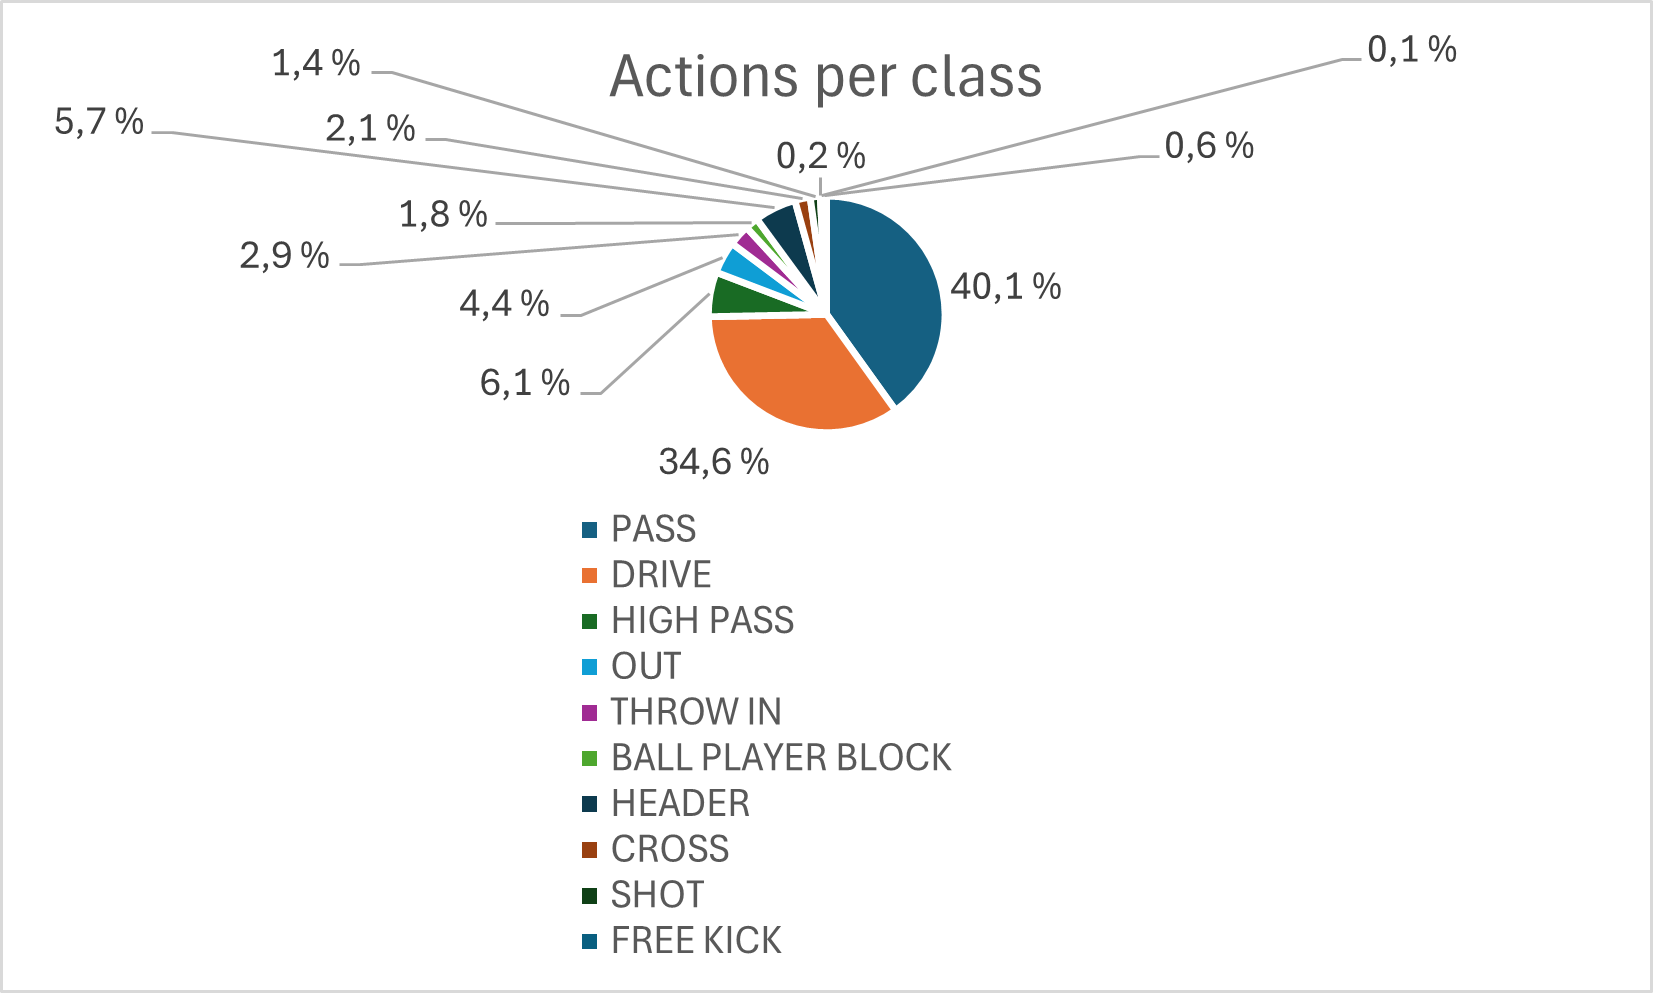
\includegraphics[width=1\linewidth]{figures/actions_per_class.png}
    \caption{Action distribution for different classes in the SoccerNet dataset for action ball spotting.}
    \label{fig:soccernet_dist}
\end{figure}


\section{Model Architectures}
\label{sec:model_architectures}

\subsection{VideoMAE-V2}
\label{ssec:videomae_v2}

\acrfull{vmae} by \textcite{wang_videomae_2023} is a self‑supervised masked autoencoder designed specifically to preprocess and compress large‑scale video data before downstream experiments. Building on the original VideoMAE, it introduces a dual‑stage masking schedule: 

\info{feature extractor (hyperparams, masking schedule)}
\begin{itemize}
    \item \emph{Sparse spatiotemporal masking} in early epochs to encourage global context learning over long clips,
    \item \emph{Dense tube masking} in later epochs to refine local motion representations.
\end{itemize}

VideoMAE has three components, embedder, encoder and decoder. VideoMAE uses cube embedding \(\Phi_{emb}\) to transform frames into sequences of tokens. It designs a tube masking strategy with ratios \(\rho \simeq 90\%\). The visible tokens are encoded by a vanilla \acrshort{vit} backbone. A decoder reconstructs the masked patches using another \acrshort{vit}\cite{wang_videomae_2023}. 
% Each frame is first partitioned into non‑overlapping $P\times P$ patches and tokenized; a binary mask tensor $M\in\{0,1\}^{T\times H/P\times W/P}$ with masking ratio up to 90\% is then generated according to the dual schedule. The visible tokens $x_{\rm vis}=x\odot(1-M)$ are encoded by a standard ViT backbone, while a lightweight three‑layer transformer decoder reconstructs only the masked patches. 
\improvement{there is some juicy math in the paper which can help the thesis seem more professional}

By dynamically varying the masking granularity, VideoMAE‑V2 achieves:
\begin{itemize}
    \item 2× faster convergence compared to VideoMAE,
    \item linear scaling to billion‑parameter models,
    \item robust transferability across action recognition, temporal localization and segmentation tasks\cite{wang_videomae_2023}.
\end{itemize}

Pre-extraction of VideoMAE-V2 embeddings significantly reduces storage and computational demands. Saving compact feature vectors instead of raw video sequences lowers I/O overhead and accelerates data loading. This approach decouples frame encoding from model training, enabling more rapid iterative experiments. As a result, overall training time decreases and resource utilization improves. \unsure{repetition?}

\subsection{\acrfull{s6}}
\label{ssec:s6}

\acrfull{ssm} offer a continuous-time representation of sequential data via a latent state \(h(t)\in\mathbb{R}^N\):
\begin{align}
    \frac{\mathrm{d}h(t)}{\mathrm{d}t} &= A\,h(t) + B\,x(t),  \label{eq:ssm_continuous1}\\
    y(t) &= C\,h(t),                                    \label{eq:ssm_continuous2}
\end{align}
where \(x(t)\in\mathbb{R}^d\) is the input, \(y(t)\in\mathbb{R}^m\) the output, and \(A\in\mathbb{R}^{N\times N}, B\in\mathbb{R}^{N\times d}, C\in\mathbb{R}^{m\times N}\) are learned parameters.  Discretizing these equations with step size \(\Delta\) yields
\begin{align}
    \bar A &= \exp(\Delta\,A), 
    & 
    \bar B &= \bigl(\exp(\Delta\,A)-I\bigr)A^{-1}B,\\
    h_k &= \bar A\,h_{k-1} + \bar B\,x_k, 
    &
    y_k &= C\,h_k,
    \quad k=1,2,\dots
\end{align}
\unsure{Do I have to reference equations in the same way figures must be referenced in a text}
VideoMamba \cite{li_videomamba_2024} builds on this framework with a \emph{Selective Scan} (\acrshort{s6}) core.  Its parameters \((\Delta, A,B,C)\) control:
\begin{itemize}
    \item \(\Delta\): temporal resolution of the recurrence,
    \item \(A\): continuous dynamics matrix,
    \item \(B,C\): input and output mappings.
\end{itemize}

By preserving a compact hidden state, Mamba approximates long-range dependencies akin to self-attention but with only \(\mathcal{O}(L)\) time/memory cost rather than \(\mathcal{O}(L^2)\) of the \acrlong{vit}.  

\subsubsection{\acrfull{vms}}
The \acrfull{vms} is a \acrfull{sota} implementation in the Papers with Code benchmark. It integrates a \acrlong{s6} optimized for long-range temporal dependencies and offers robust performance across various video event detection tasks. 

\subsubsection{RDFA-S6}
The RDFA-S6 architecture extends the \acrshort{vms} core with recurrent mechanisms, yielding improved temporal representation capacity in benchmarks of \acrfull{tal}. Empirical evaluations reveal that RDFA-S6 achieves slightly higher mean average precision, indicating its superior performance in event localization benchmarks on THUMOS-14, ActivityNet, FineAction and HACS.

Although RDFA-S6 demonstrated marginally superior accuracy, its adoption was hindered by limited documentation compared to the well-supported \acrlong{vms}. Consequently, \acrshort{vms} remained the primary model for empirical evaluation within this study. 


\subsection{\acrfull{tdeed}}
\label{ssec:tdeed}

\acrfull{tdeed} is a deep learning architecture designed to address the challenge of \acrfull{pes} in sports videos. This model improves token discriminability while leveraging multiple temporal scales, thereby ensuring high-resolution event localization. The architecture consists of three main components: a feature extractor, a temporally discriminant encoder-decoder, and a prediction heads\cite{xarles_t-deed_2024}.

The feature extractor generates per-frame feature representations. It employs a RegNetY-based backbone with \acrfull{gsf} modules, integrating local temporal context while maintaining spatial information. Given an input frame sequence of shape \(\mathbb{R}^{L \times H \times W \times 3}\), the extracted feature representation is formulated as:

\[
z \in \mathbb{R}^{L/{k^j \times d} }
\]

The encoder-decoder architecture enables processing across multiple temporal scales, capturing events that require varying amounts of temporal context. The encoder enhances token discriminability using \acrfull{sgp} layers, which mitigate similarity issues commonly present in adjacent frames. The temporal dimension is downscaled through max-pooling, followed by an upsampling process in the decoder. Skip connections are integrated into the decoder using the \acrshort{sgp}-Mixer layer, which aggregates features from different temporal scales while preserving fine-grained temporal details.

The prediction head consists of two components: a classification head and a displacement head. The classification head predicts event occurrences per frame using a softmax function, while the displacement head improves predictions by estimating the precise event frame within a given radius. This ensures robust event localization even when slight spatial or temporal differences exist.


T-DEED is trained end-to-end using a multi-task loss. The loss comprises a weighted cross-entropy loss \(\mathcal{L}_c\) and a displacement loss \(\mathcal{L}_d\), defined as

\[
\mathcal{L} = \frac{1}{L}\sum_{l=1}^{L}\Big(\mathcal{CE}_{w}(y_l^{c},\hat{y}_l^c) + \operatorname{MSE}(y_l^{d},\hat{y}_l^d)\Big).
\]

Here, \(y_l^{c}\) is the one-hot encoding of the event in frame \(l\). The probability distribution at frame \(l\) is denoted by \(\hat{y}_l^c\). Similarly, \(y_l^{d}\) and \(\hat{y}_l^d\) represent the ground truth and predicted displacements, respectively.

\paragraph{Implementation Details} The experiments use a T-DEED implementation adapted for the SoccerNet challenge. Embeddings are computed offline following the original method. Event spotting performance is evaluated using mean Average Precision at IoU thresholds \(\{0.1,0.3,0.5\}\).


\section{Training Details}
% optimizer, learning rates, augmentation, early‐stopping, etc.

In this study, we evaluated both \acrshort{vms} and RDFA-S6 architectures, balancing performance and ease of use. RDFA-S6 achieved slightly higher event localization accuracy on benchmarks, yet its documentation and setup complexity introduced reproducibility challenges. By contrast, the \acrshort{vms} implementation provided comprehensive THUMOS dataset annotations, robust download links, and a well-structured run script. These features facilitated an easier integration into the experimental pipeline. Consequently, \acrshort{vms} was chosen as primary model, given its superior usability and reliable performance.

In the experiments, all training hyperparameters and architectural settings are specified in external configuration files, ensuring reproducibility and transparency. An early stopping mechanism based on validation loss is used, which halts training when performance improvements plateau and/or decrease. While no explicit data augmentation pipelines are utilized during model fitting, selective augmentation techniques are available and configurable through the same files if needed.

\section{Bayesian Hyperparameter Optimization}
\label{sec:bayesian_optimization}

I employed \acrshort{wandb} Sweeps to perform Bayesian Optimization for efficient hyperparameter tuning.  A Gaussian Process surrogate modeled the validation \acrshort{map} as a function of learning rate, weight decay, and hidden dimension. Uniform and log-uniform priors were defined over each hyperparameter in the sweep configuration .YAML file. The expected improvement acquisition function guided the selection of promising hyperparameter combinations. 70 trials were run in three iterations. THe 70 runs were in parallel\footnote{All runs were run as individual trainings, and had nothing to do with each other except the \acrshort{wandb} agent designing parameters. } across multiple GPUs to explore the search space while minimizing wall-clock time. All metrics and configuration parameters were logged to \acrshort{wandb}, enabling real-time monitoring and reproducibility. 

\section{visualisation}

idk if this deserves a section or subsection but last year the boys had it. i might define more visualisations while I write discussion and results

\section{\acrshort{vms} Evaluation Protocol}
When evaluating \acrshort{vms} performance, the the 50\% \acrshort{map} criterion from the SoccerNet benchmark is adopted, which employs a $\pm 1s\,$ tolerance window for event matching. Since the \acrshort{vms} model is validated against fixed‐length intervals of $L = 2\,$s, achieving $\mathrm{IoU}\ge0.5$ requires an overlap of at least $L/2 = 1s\,$.

Let $t^*$ denote the ground‐truth event time and $t_p$ the predicted center. The predicted interval is
\[
    [\,t_p - L/2,\;t_p + L/2\,]
    = [\,t_p - 1,\;t_p + 1\,].
\] 
The IoU condition
\[
    \mathrm{IoU}
    = \frac{\text{overlap}}{\text{union}}
    \;\ge0.5
    \quad\Longrightarrow\quad
    \text{overlap}\ge1
    \quad\Longrightarrow\quad
    |t_p - t^*|\le1
\]
ensures that the predicted center $t_p$ lies within one second of the true event time.

I measured runtime directly from \acrshort{wandb} logs, as the platform automatically records wall-clock time for each training run. However, these values vary according to the assigned GPU model. To ensure fair comparisons, all measurements were standardized on a single GPU type. 

\section{Environment} 

multiple environments
i used python, but environments also had CUDA code, and c++ code. 
different repositories for different experiments
is vms environment or tool?
can I just put environments in appendix? environments are stored in wandb if i understand it correctly with version control